\setAuthor{Andreas Valdmann}
\setRound{piirkonnavoor}
\setYear{2010}
\setNumber{G 8}
\setDifficulty{7}
\setTopic{Geomeetriline optika}

\prob{Hajuti}
Mõnedes valgustites kasutatakse valguse hajutamiseks joonisel kujutatud ristlõikega
pleksiklaasist plaati. Valgus langeb selle siledale poolele ja läbib hajuti vaid juhul, kui
langemisnurk on suurem kriitilisest nurgast $\alpha_\mathrm{kr}$. Leidke nurga $\alpha_\mathrm{kr}$ väärtus. Pleksiklaasi
murdumisnäitaja $n=\num{1,5}$. Kõik sakilise poole tahud on \num{45}-kraadise nurga all sileda poole pinna
suhtes.
\begin{center}
	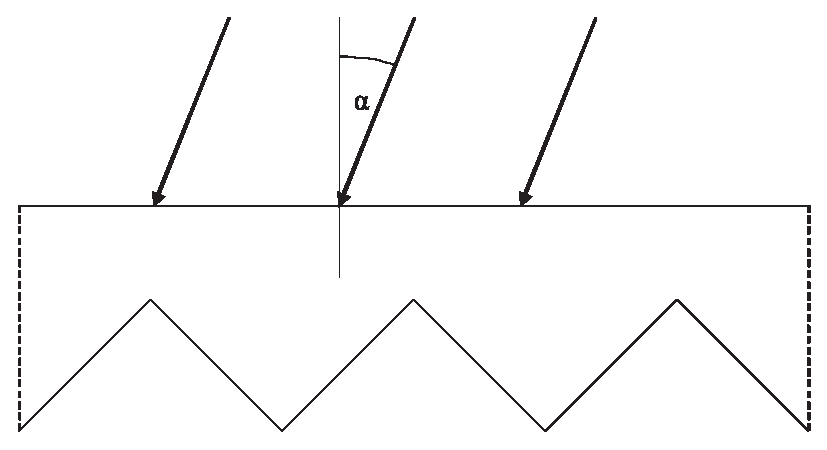
\includegraphics[width=0.475\textwidth]{2010-v2g-08-hajuti.eps}
\end{center}

\hint
Kriitilise langemisnurga all on valgus sakilisel poolel täieliku sisepeegeldumise piiril. Selleks, et antud tingimust langemisnurgaga siduda on kasulik joonestada suur ja selge joonis.

\solu
\begin{center}
	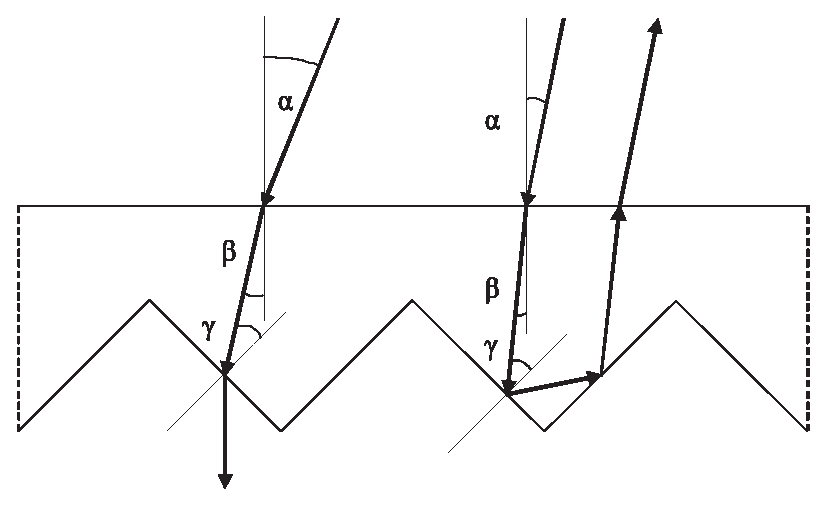
\includegraphics[width=0.6\textwidth]{2010-v2g-08-hajuti_lah.eps}
\end{center}

Valgus läbib hajuti, kui nurk $\gamma$ on väiksem täieliku sisepeegeldumise nurgast. Kriitilisel juhul $\sin(\gamma_\mathrm{kr})=1/n$. Kuna $\beta=\ang{45}-\gamma$, siis $\beta_\mathrm{kr} = \ang{45}-\arcsin(1/n)$. Nurkade $\alpha$ ja $\beta$ vahel kehtib murdumisseadus $\sin(\alpha)/\sin(\beta)=n$. Seega
\[
\alpha_\mathrm{kr}=\arcsin(n\sin(\ang{45}-\arcsin(1/n))).
\]
Vastuse saab viia kujule
\[
\alpha_\mathrm{kr}=\arcsin\left[\frac{\sqrt2}{2}(\sqrt{n^2-1}-1)\right] = \ang{4.8}.
\]
Kriitilisest väiksema $\alpha$ korral (vt parempoolsemat kiirt) on tagasi pöörduv kiir paralleelne hajutile langenud kiirega. Kiirte käigu pööramisel selgub, et tulemus ei muutu, kui esimene sisepeegeldus toimub $45$-st kraadist suurema nurga all. Sel juhul toimub nurga $\gamma$ all teine sisepeegeldus.
\probend